\chapter{Subsistema de recepción e ingesta}

\section{Arquitectuta del subsistema}

\begin{figure}[!htb]
	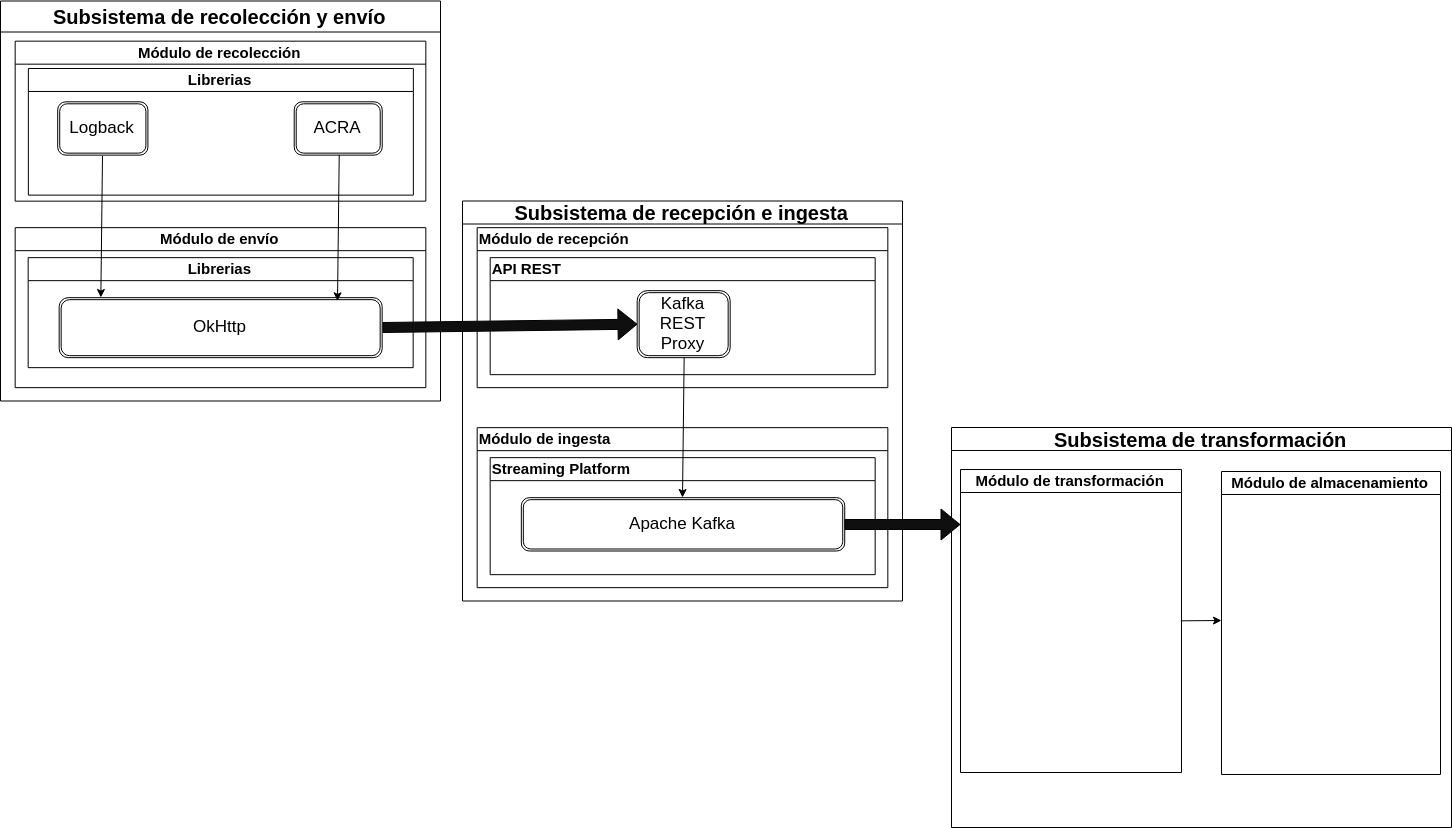
\includegraphics[width=\linewidth]{Moduloss-subrecing.png}
	\caption{Vista general del subsistema de recolección y envío}
	\label{fig:subrecing}
\end{figure}

El subsistema de recepción e ingesta está formado por dos módulos, los cuales actúan fuera del dispositivo ubicuo. Esta es una división a nivel lógico y existe para reducir a problemas más simples el problema general, aunque nada impide que una herramienta implemente dos módulos. En la figura \ref{fig:subrecing} se puede ver como se relacionan los módulos y las herramientas del subsistema. Las flechas indican el sentido del flujo de datos.

\subsection{Módulo de recepción}

El módulo de recepción en el encargado de recibir los eventos que le envía el módulo de envío y de enviárselos al módulo de ingesta. Este módulo no almacena de forma persistente los eventos recibidos.
\\\\
Se ha añadido este módulo para centralizar a un único punto de entrada y tener una metodología de envío universal para todos los dispositivos ubicuos de la empresa. De esta manera, también se facilita el que nuevos dispositivos ubicuos, diferentes a los que la empresa utiliza, puedan integrarse con el sistema.

\subsection{Módulo de ingesta} 

El módulo de ingesta es el encargado de recibir los eventos del módulo de recepción y dejar a disposición los datos al módulo de transformación. Este módulo almacena tanto de forma persistente como volátil los eventos recibidos.
\\\\
Se ha añadido un módulo entre el módulo de recepción y el módulo de transformación por cuatro razones:

\begin{enumerate}
	\item Permitir el reprocesado de los datos.
	\item No saturar al módulo de transformación.
	\item No perder eventos si el módulo de transformación está caído.
	\item Facilitar la integración de nuevos módulos.
\end{enumerate}

Al añadir un módulo que almacene los datos sin procesar antes del módulo de transformación, se permite que el módulo de transformación pueda volver a consumir datos que ya había procesado antes. Tal módulo querría reprocesar los datos por algún error humano en el programa que se encarga de transformarlos. Estos datos sin procesar no se almacenarán por siempre en el módulo de ingesta, sino que se irán eliminado del módulo siguiendo una política de limpieza establecida por el administrador del sistema.

Puesto que el módulo de ingesta sirve los datos para que sean consumidos, el módulo de transformación los consume cuando puede, de esta manera si estaba caído o estaba saturado, y puesto que módulo de ingesta almacena los datos de forma persistente, los consumirá cuando vuelva a estar arriba o pueda consumirlos.
\\\\
Añadir este módulo de ingesta facilita la integración de nuevos módulos ya que transforma parcialmente los datos recibidos para que sean compatibles con los diferentes módulos que se le puedan acoplar. A parte, facilita el enrutamiento de los datos hacia los diferentes módulos que se le quieran acoplar.

\section{Estructura del subsistema}

\subsection{Módulo de recepción}
El módulo de recepción lo integra una API REST que es capaz de recibir los eventos y enviarlos al módulo de ingesta. Se ha escogido una API REST, puesto que la comunicación mediante peticiones REST permite una fácil integración con los dispositivos ubicuos. Utilizar una API REST también ayuda a que el sistema se pueda integrar rápidamente con nuevos dispositivos ubicuos diferentes a los que usa actualmente la empresa.

\subsection{Módulo de ingesta}
El módulo de ingesta lo integra una streaming platform, una especie de buffer que almacena los datos sirviéndolos para que otro módulo los consuma. Suple las funciones de un message broker\cite{Tfg:messagebroker} y le añade ciertas funcionalidades. Esta streaming platform es capaz de recibir los eventos y almacenarlos en memoria y en disco.


\section{Herramientas utilizadas}

%%TODO: Preguntar a Xavi como poner la fuente
\subsection{Módulo de ingesta}
Para el módulo de ingesta se ha escogido utilizar Apache Kafka\cite{Tfg:kafka}, a parte de porque posee las funcionalidades requeridas, por las siguientes razones:

\begin{itemize}
	\item Compatibilidad: Ofrece una gran compatibilidad con las posibles herramientas a utilizar en el módulo de transformación, aparte de con otras herramientas de otros posibles módulos que se quieran acoplar.
	
	\item Documentación: Existe una documentación extensa sobre la herramienta y la comunidad es bastante activa.
	
	\item Confiabilidad: Kafka es capaz de tener múltiples consumidores y productores subscritos. En caso de fallo de alguno de los nodos componentes de Kafka, es capaz de balancear automáticamente los consumidores y los productores a nodos componentes funcionales. Aparte, Kafka replica los datos que recibe entre los diferentes nodos componentes.
	
	\item Durabilidad: Los mensajes que recibe Kafka los almacena en disco, por lo que aparte de la replicación de datos que hace el propio Kafka, es fácil replicar los datos hacia otro sistema.
	
	\item Escalabilidad: Kafka es capaz de escalar rápido, de forma fácil y en caliente ya que es un sistema distribuido.
	
	\item Rendimiento: Debido al uso de los recursos que hace Kafka, es capaz de ofrecer un throughput elevado tanto a productores como consumidores.
\end{itemize}

\subsection{Módulo de recepción}
Para el módulo de ingesta se ha escogido utilizar Kafka Rest Proxy\cite{Tfg:kafkarestproxy}, a parte de porque posee las funcionalidades requeridas, la elección de esta herramienta ha dependido de la elección de la herramienta del módulo de ingesta, ya que se ha tenido que buscar una herramienta que sea integrable con Apache Kafka. La herramienta escogida ha sido creada por los mismos creadores que Apache Kafka y la integración está completamente asegurada. A parte de la integración, esta herramienta nos aporta ciertos beneficios de confiabilidad y escalabilidad que serán más evidentes en su despliegue.

\section{Configuración del subsistema}

\subsection{Módulo de recepción}

En el Capítulo \ref{cap:despligue} se hablará con más detalle de que este módulo a parte de máquinas tiene un balanceador de carga que distribuye el trabajo entre las máquinas. Configurar ese balanceador de carga también forma parte de la configuración de este módulo. A ese balanceador se le ha tenido que decir que las peticiones REST que vengan por un puerto en concreto las redirija a las máquinas que forman el módulo de recepción.
\\\\
A las máquinas que forman el módulo de recepción se le ha tenido que configurar el destino de los mensajes recibidos, es decir, que envíen los mensajes que reciben del módulo de envío al módulo de ingesta. También se le ha tenido que dotar de una id única para que el módulo de ingesta reconozca las máquinas.

\subsection{Módulo de ingesta}

El módulo de ingesta tiene una forma particular de almacenar los datos. Almacena los datos en \textit{topics}, los \textit{topics} son similares a las tablas en SQL. Se han creado dos \textit{topics}, el \textit{topic} logs, donde se almacenarán los logs, y el \textit{topic} crashlogs donde se almacenarán los crashlogs. Los \textit{topics} se dividen en particiones para explotar al máximo el paralelismo y permitir que diversas máquinas consuman diferentes particiones del mismo \textit{topic}. Estas particiones se pueden replicar entre las máquinas con el fin de aumentar la durabilidad y la confiabilidad del sistema. Por lo que en resumen la configuración escogida de los \textit{topics} es la siguiente:

\begin{itemize}
	\item Topic \textit{logs}, 3 particiones, 3 replicas de cada partición. De esta manera 3 máquinas pueden consumir los datos a la vez y pueden fallar 2 máquinas del cluster que aún los datos serán accesibles.
	\item Topic \textit{crashlogs}, 3 particiones, 3 replicas de cada partición. De esta manera 3 máquinas pueden consumir los datos a la vez y pueden fallar 2 máquinas del cluster que aún los datos serán accesibles.
\end{itemize}

A parte, el sistema nos permite definir una política de limpieza para los datos almacenados. Se ha establecido que los datos permanezcan almacenados en el sistema de forma persistente una semana. Es un tiempo más que suficiente para detectar un mal procesado y tener que volver a reprocesar los datos.

Como en Kafka se puede forman un cluster de máquinas, a cada máquina se le ha tenido que configurar a qué cluster pertenece.




